\section{Choosing Sound Classes}
Based on some of the previous works by \cite{Stowell2010} and \cite{QBBB} a set of 3 basic beatboxing sounds have been chosen for this experiment. The first of them is the kick drum, which is also known as the base drum because of its deep-sounding nature. The spectrum of the kick drum lies in the lower frequencies as seen in figure \ref{fig:kick-wave}. The second sound is the snare drum and we have been focussing on the k-snare as opposed to the p-snare, which is performed with an initial k-sound. Lastly the hi-hat cymbal was chosen, which has a frequency spectrum a bit higher than the snare as can be seen in figure \ref{fig:snare-wave} and \ref{fig:hihat-wave}.

\begin{figure}[h]
	\centering
	\begin{subfigure}[b]{0.275\textwidth}
		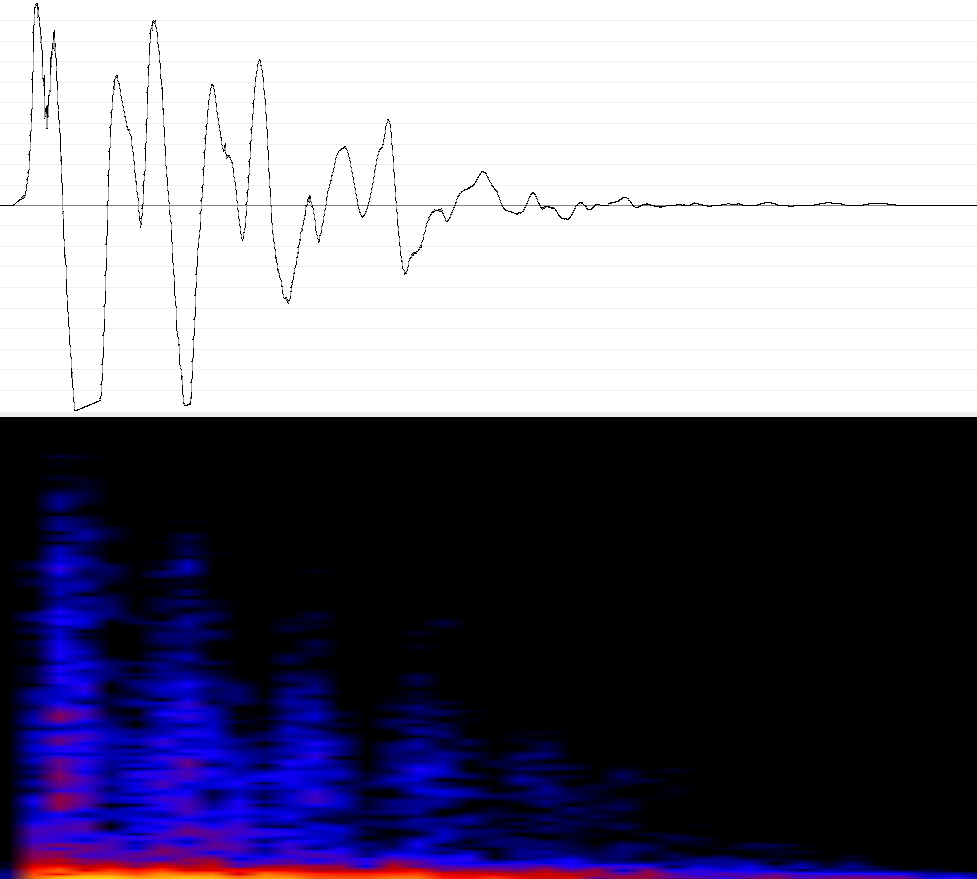
\includegraphics[width=\textwidth]{fig/Kick-wave.png}
		\caption{Kick drum}
		\label{fig:kick-wave}
	\end{subfigure}
	\begin{subfigure}[b]{0.275\textwidth}
		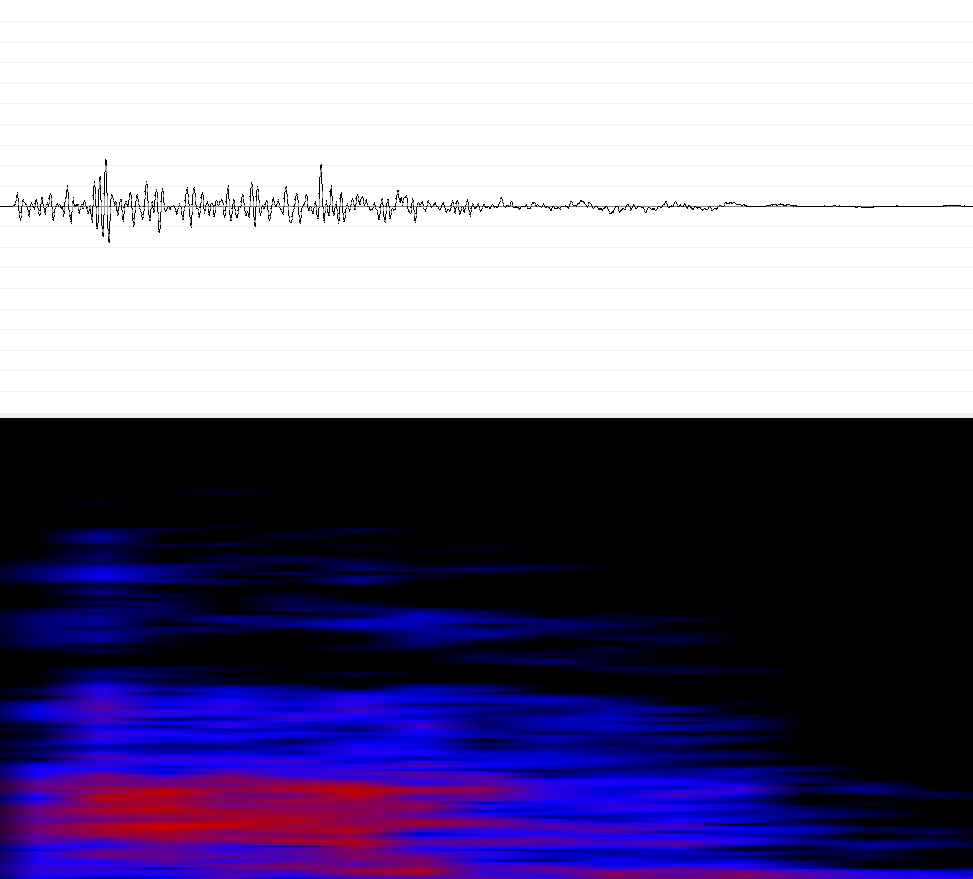
\includegraphics[width=\textwidth]{fig/Snare-wave.png}
		\caption{Snare drum}
		\label{fig:snare-wave}
	\end{subfigure}
	\begin{subfigure}[b]{0.35\textwidth}
		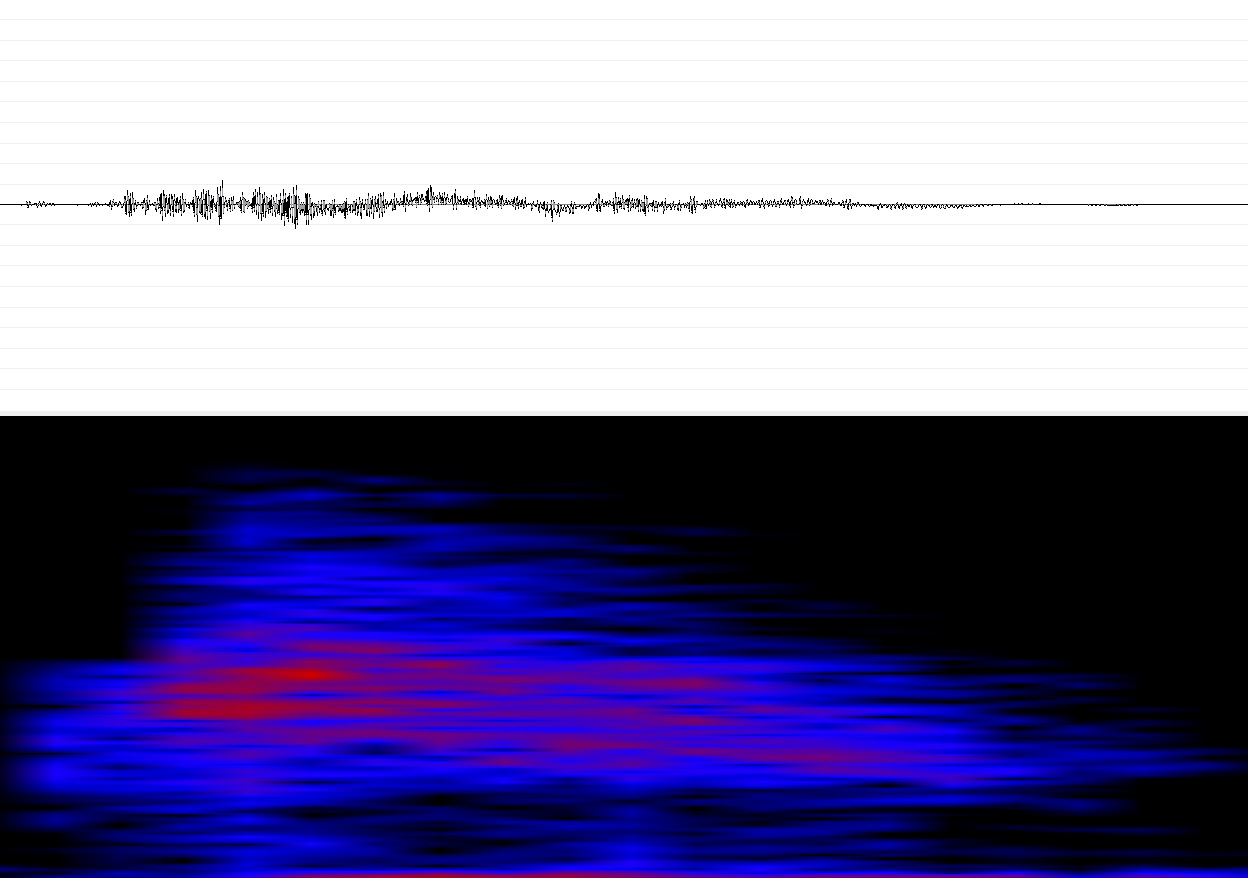
\includegraphics[width=\textwidth]{fig/Hihat-wave.png}
		\caption{Hi-hat}
		\label{fig:hihat-wave}
	\end{subfigure}
	\caption{A presentation of 3 beatboxing sounds' waveform (top) and spectrogram
	\label{fig:chosen-sounds} (bottom).}
\end{figure}

What we can see from these waveforms and spectra is that the kick drum does differ significantly in its frequency content in relation to the snare and hi-hat. The snare and hi-hat does initially seem to have a clear difference in their frequencies, however they do not seem to lie in a very concentrated area of the spectrum, indicating that they might prove difficult to distinct from each other based on the frequency content.